\chapter{Manipulando GUI}

O PD foi desenvolvido utilizando um modelo que separa a apresentação das
funcionalidades.
Isto rola com 2 linguagens de programação: C para a engine e tcl/tk para as GUI.
GUI e engine se comunicam por um socket que permite, inclusive, que a engine
do PD seja executada em uma máquina e a GUI em outra.

% \url{http://puredata.info/docs/guiplugins/GuiPluginsAPI/}

% -----+-----+-----+-----+-----+-----+-----+-----+-----+-----+-----+-----+-----+
%      |     |     |     |     |     |     |     |     |     |     |     |     |
% -----+-----+-----+-----+-----+-----+-----+-----+-----+-----+-----+-----+-----+
\section{Iniciando no Tcl/Tk}
O Tcl (Tool Command Language) é uma linguagem de programação dinâmica bastante poderosa e simples de ser utilizada. 
Tk é um conjunto de ferramentas para construção de GUI de aplicações desktop e é a GUI padrão não apenas do TCL mas 
de várias outras linguagens e pode ser executada nativamente em vários sistemas operacionais modernos como Windows,
 Mac OS X, Linux, entre outros \footnote{Visite: http://www.tcl.tk/ para maiores informações}.

O Tk possui vários objetos prontos para GUI como botões, labels, janelas, checkbox, entre outros. Os objetos criados
devem ser armazenados em uma variável. Toda variável em Tk possui um nome que inicia com ponto (.). Após criar o objeto
e definir seus atributos, basta que o mesmo seja empacotado (pack).

\begin{lstlisting}
label .hello -text "Hello World"
pack .hello
\end{lstlisting}

Uma vez que um programa tk esteja pronto, basta salvá-lo com a extensão .tcl e utilizar um interpretador para executá-lo.
Um exemplo deste interpretador no Linux é o wish. Assim, salvando o exemplo anterior com o nome de helloWorld.tcl e executando

\begin{lstlisting}
wish helloWorld.tcl
\end{lstlisting}

Teremos o resultado:
\begin{figure}[ht!]
	\centering
	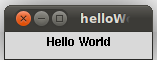
\includegraphics[width=0.7\textwidth]{helloWorld}
	\caption{Hello World no Tcl/Tk}
\end{figure}

No diretório tk deste tutorial temos exemplos mais interessantes de GUI com Tk mas a prática desta linguagem
vai além do escopo deste tutorial. Um tutorial mais completo de Tcl/Tk pode ser encontrado em 
\footnote{http://www.bin-co.com/tcl/tutorial/} e uma lista dos objetos e parâmetros pode ser encontrada em
\footnote{http://www.tkdocs.com/widgets/index.html}.


